\chapter{Experimental setup}
As this thesis deals with the manipulation of the magnetization of antiferromagnets via optically driven thermal and electronic excitations \cite{song_how_2018} the observed dynamics take place on the ultrafast timescale and a time-resolved technique capable of femtosecond resolution is needed.
This is achieved using a pulsed femtosecond laser.
All measurements are carried out using the table-top setup as established by Mertens et al. \cite{mertens_wide_2020}.

\subsubsection*{Pump-probe measurements}
In the frame of this thesis most of the measurements are done via pump-probe spectroscopy, as we focus on the ultrafast time evolution of the antiferromagnetic systems after an optical excitation.
Two pulsed laser beam are used to take time resolved measurements, the pump and the probe.
The pump pulse acts as a perturbation and excites the system causing a change in its ordered structure.
The probe pulse is used to probe the perturbed system and to extract information about the origin of the change, which translates to a MO effect happening in turn causing measurable modification of the probe pulse such as the rotation of polarisation or ellipticity.
By shifting the time delay between these two laser pulses it is possible to figuratively scan the system's response in the time domain.
A delayline with a minimal stepsize of \qty{75}{nm} in the pump path enables the control of the time delay down to \qty{50}{fs} limited only by the pulse duration itself.
\begin{figure}[ht]
    \centering
    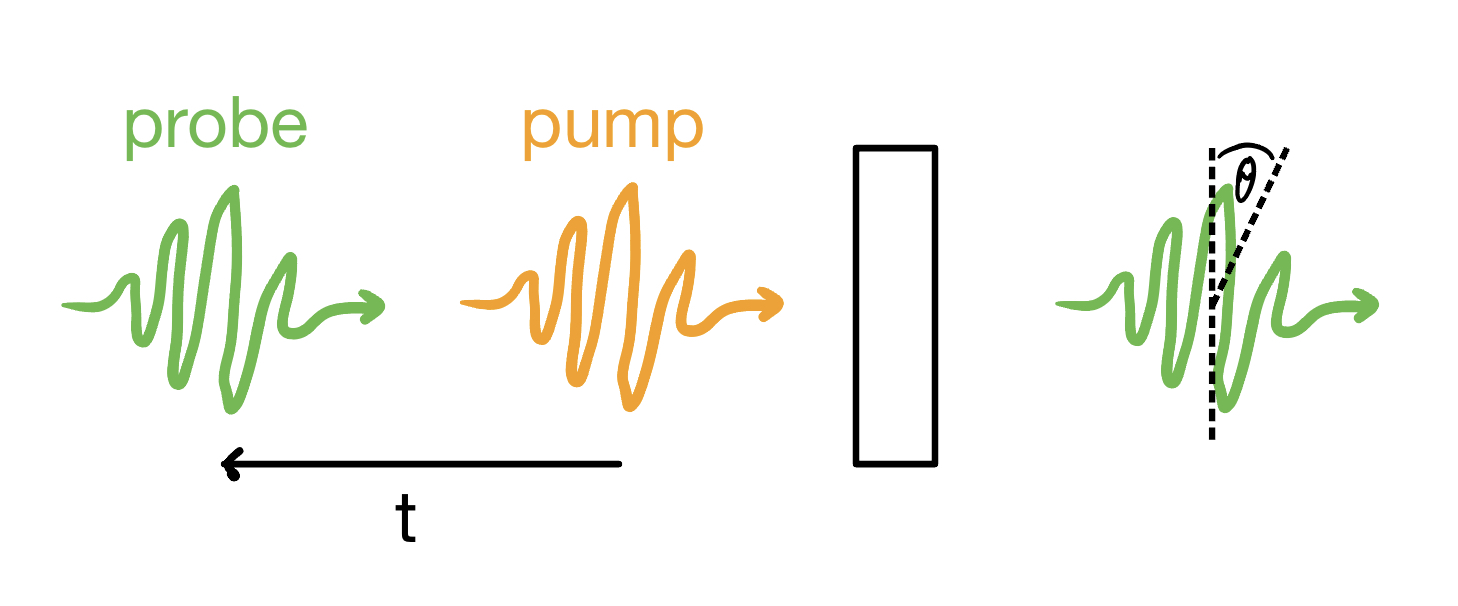
\includegraphics[width=0.6\textwidth]{pictures/pump_probe.jpeg}
    \caption{Schematic depiction of transmission pump-probe measurement.}
    \label{fig:pump_probe}
\end{figure}

\subsubsection*{Laser system}
Here a commercial ytterbium-based pulsed femtosecond laser (PHAROS) made by Light Conversion with a central wavelength of \qty{1028}{nm}, a pulse duration of about \qty{300}{fs} and a power of \qty{20}{W} is used.
With a repetition rate of \qty{50}{kHz} each pulse carries an energy of \qty{100}{\uJ}.
The Pharos output is split into two beams with \qty{7}{W} and \qty{13}{W}, of which the first one is designated to be the probe and the second to be the pump beam.
To ensure a separate tunability in wavelength of the two beams each one is fed into an optical parametric amplifier (OPA) Orpheus.
The OPA consists of a series of non-linear optics mounted on motorized stages, containing among others white light generation (WLG) and difference frequency generation (DFG).
The former of which makes it possible to select a specific signal frequency to amplify via the DFG process.
\begin{figure}[ht]
    \centering
    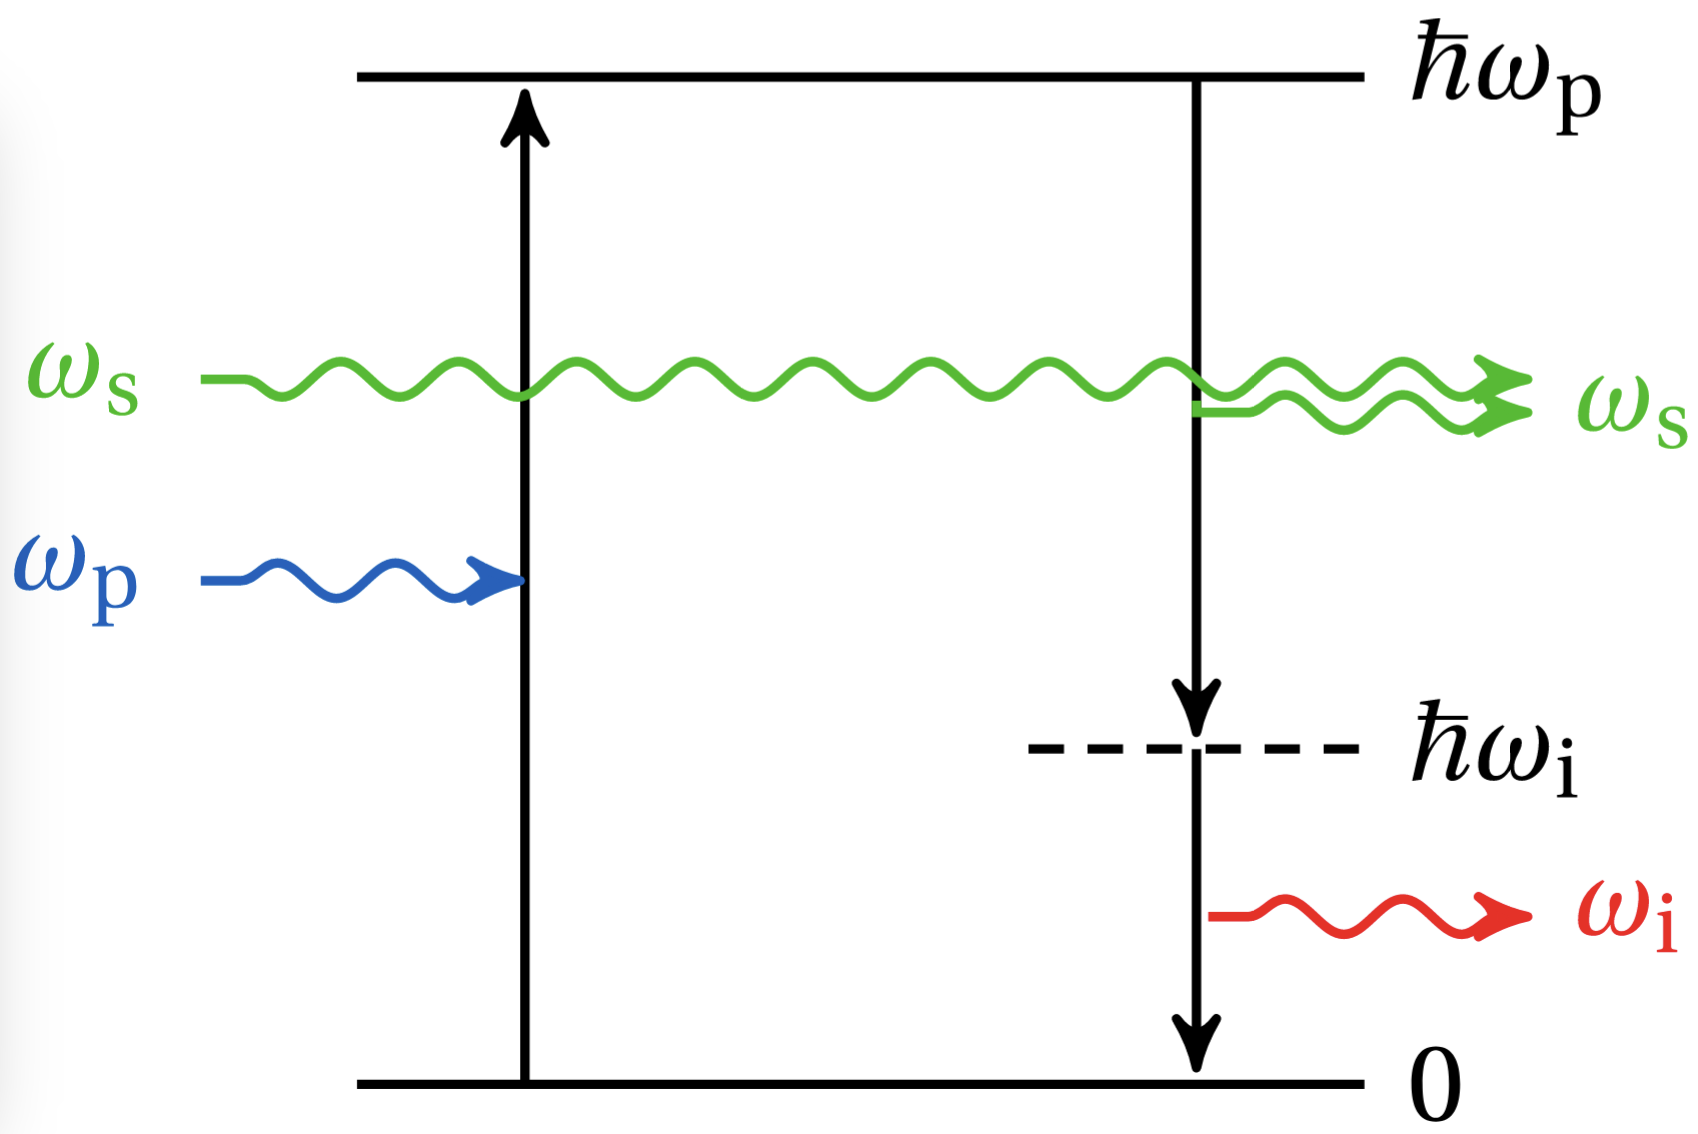
\includegraphics[width=0.5\textwidth]{pictures/OPA.png}
    \caption{Illustration of energetic transisions involved in the process of optical parametric amplification.}
    \label{fig:OPA}
\end{figure}
As can be seen in \autoref{fig:OPA} a pump beam is necessary to amplify the signal beam.
Another beam called idler is created as a byproduct, so that the following relation holds:
\begin{equation*}
    \omega_{\text{p}} = \omega_{\text{s}} + \omega_{\text{i}}
\end{equation*}
Before the OPA for the pump an electro optical modulator is placed only letting every second pulse pass.
This has the effect that half of the probe pulses encounter an unpumped sample, which sets a baseline for the detected signal.
The OPA also incorporates an internal compressor for the idler beam.
To compensate for the signal beam, its path can be manually adjusted via a quick replacement of mirrors to go through an external compressor.
Making up the last component of the stationary laser system is the external second harmonic generator (LYRA).
It extends the spectrum by twice reaching from \qty{0.5}{eV} to \qty{3.5}{eV}. 
\begin{figure}[ht]
    \centering
    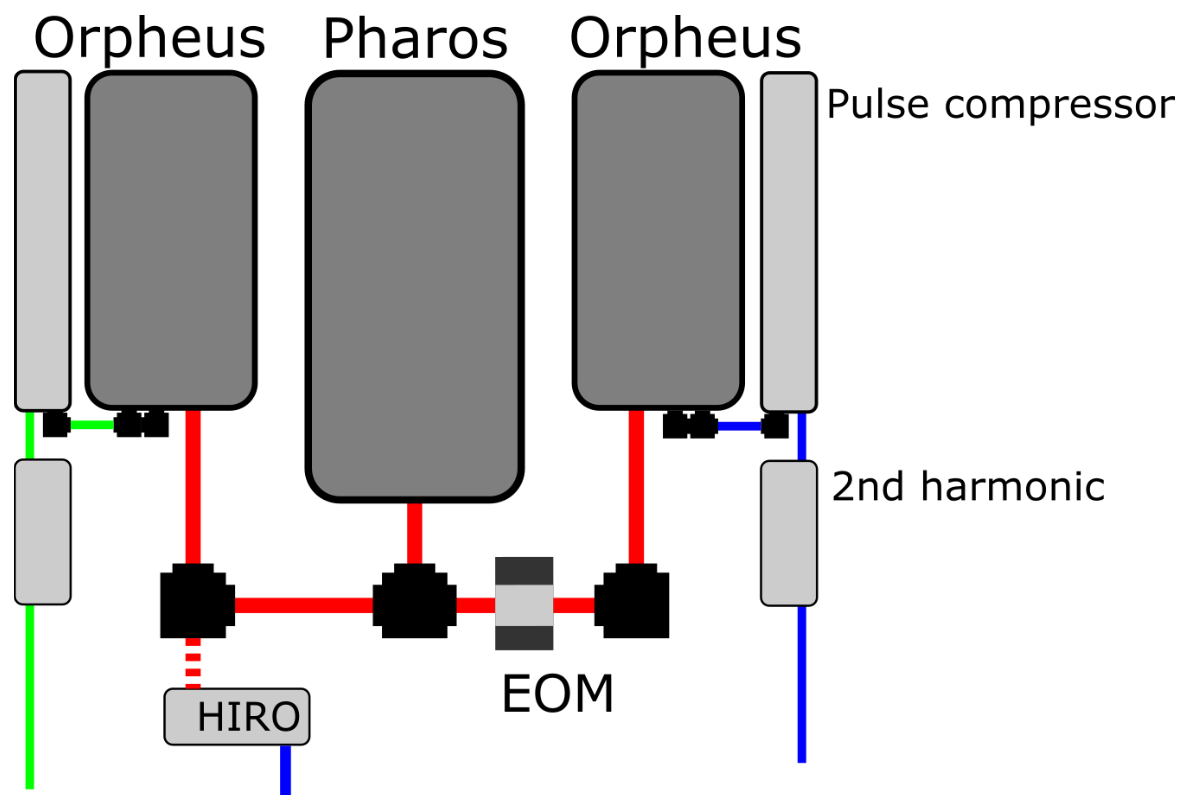
\includegraphics[width=0.65\textwidth]{pictures/laser_system.png}
    \caption{Schematic of the laser system containing labelled parts.}
    \label{fig:laser_systems}
\end{figure}
With the exception of the external compressor, the system can be operated with the corresponding desktop application and automatically adopts the typed-in wavelength.

\subsubsection*{Optical path}
As already mentioned above, a delayline is stationed in the pump beam path.
The pump travels the distance between the mirror and the delayline four times, which accounts for a factor of $\frac{4}{c}$ between the time delay and the shifted distance.
The laser light is horizontaly polarized to the plane of the table [PHAROS manual], so as an attenuator for the high peak power, a linear polarizer cube in combination with a $\frac{\lambda}{2}$-waveplate is used.
To vary the transmitting intensity the waveplate is rotated and to vary the angle of the light polarization for polarization dependent measurements an additional $\frac{\lambda}{2}$-waveplate is installed behind the attenuator.
Both the beams are then focused either by lenses or an objective on a common point on the sample surface, where a spatial overlap is achieved by using the computer-controlled piezo-driven mirror-holder from Newport.
% It is possible to use this system in the collinear, pump and probe are parallel, or the transversal, angle between pump and probe, scheme.
% The decision which geometry to incorporate is made based on the direction of the anisotropy.
Furthermore the setup can be adjusted for reflective or transmissive measurements.
The transmissive measurements being the more straightforward ones to implement wheras the reflective ones require the use of a beamsplitter to guide the light to the detection branch.

The sample is mounted in a open-loop cryostat requiring a steady flow of helium to reach and hold a desired temperature, which is essential for measurements exploring phase diagrams.
A magnetic valve controls the cross section of the supply pipe and thus the quantity of helium being pumped through the cryostat.
To maintain a specific steady temperature a heater governed by a PID controller is in thermal contact with the sample holder.
The cryostat itself is inserted inside a closed-loop, helium-cooled, superconductive magnet generating up to $\pm\qty{9}{T}$ at the sample position normal to the sample plane.
This allows for magnetic field dependence measurements, as well as for recording of hysteresis curves.
The sample stage has three axis and can be computer-controlled down to a stepsize of \qty{1}{nm} to shift to an exact position.

\subsubsection*{Data aquisition system}
MO effects typically induce a rotation of the polarization or ellipticity in the incident light and as most of the observed samples in the context of spintronics are rather thin, the change in the probe light often amounts to only a few mrad.
To overcome this issue, a specialised technique called balanced photodetection is used suppressing the background noise while simultaneously amplifying the difference between two incoming optical signals.
Firstly, the reflected or transmitted probe beam is guided through a $\frac{\lambda}{2}$-waveplate and a Wollaston prism.
The prism splits the light $I$ in two linearly polarized rays $I = I_p + I_s$ with their polarizations perpendicular to each other as depicted in \autoref{fig:balanced_detection}.
\begin{naligned}
    E_s &= E \cos\left(\sfrac{\pi}{4} + \theta\right) \\
    E_p &= E \sin\left(\sfrac{\pi}{4} + \theta\right)
    \label{eqn:balance}
\end{naligned}%
The waveplate is used to tilt the polarization of the light to such a degree that both of the rays hit the photodetector with the same intensity.
From this equilibrium position with a now switched on, previously arriving pump pulse, the polarisation of the probe gets rotated by an angle $\theta$.
This changes the ratio between the two photocurrents, which get converted into voltage and whose difference then gets amplified via operational amplifiers.
\begin{figure}[ht]
    \centering
    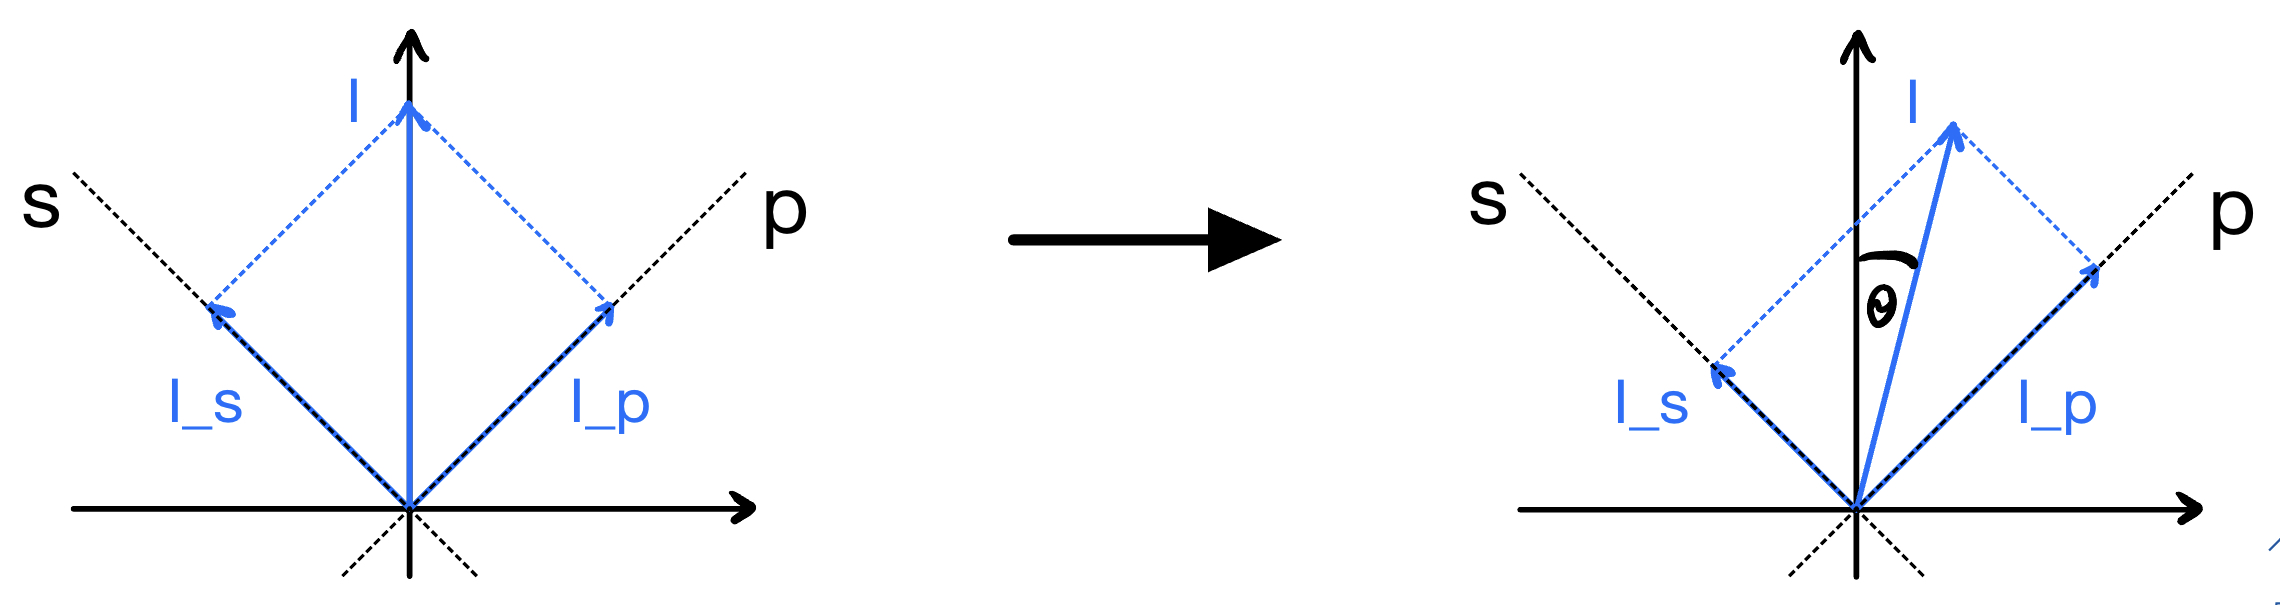
\includegraphics[width=\textwidth]{pictures/balanced_detection.jpeg}
    \caption{Representation how the incoming light gets split by the prism into two equally intense linearly polarized rays and how the subsequent rotation of polarisation materializes in the difference between s- and p-polarized light intensity.}
    \label{fig:balanced_detection}
\end{figure}
As the light is measured with a photodetector the incident light power is proportional to the generated current which in turn is proportional to the converted voltage and thus the signal observed on the computer.
Using this and \autoref{eqn:balance} the proportional  relation
\begin{equation}
    S \propto E_s^2 - E_p^2 \approx 2 E^2 \theta
\end{equation}
between a small angle $\theta$ and the signal $S$ can be derived.